% ==========================================================
% PREAMBLE
\documentclass[english,11pt,a4paper]{scrartcl}
\usepackage[T1]{fontenc} % --------------| More characters.
\usepackage[utf8]{inputenc} % -----------| Direct use of scandinavian letters.
\usepackage{float} % --------------------| More options for floats.
\usepackage{graphicx} % -----------------| Support more image formats.
\usepackage{booktabs} % -----------------| Better-looking tables.
\usepackage{tabularx} % -----------------| Better tables
\usepackage{subfig} % -------------------| Subfigures.
\usepackage[a4paper]{geometry} % --------| Adjusting page margins. % showframe
\usepackage{amsmath,amssymb,amsfonts} % -| Various math, including eqref.
\usepackage{xcolor} % -------------------| Allows defn. of custom colors.
\usepackage{babel}
\usepackage{url}
\usepackage{enumitem} % -----------------| Used to adjust spacing in lists
% \usepackage[boxed]{algorithm2e} % -------| Used to typeset algorithms
% Breaks with \bibliography on bhome

% XY-PIC. USED FOR CREATING ILLUSTRATIONS.
\input xy
\xyoption{all}

% STYLING CAPTIONS
\usepackage{caption}
\captionsetup{margin=10pt,font=small,labelfont=bf}
% \usepackage{fancyhdr} % -----------------| % NOT WITH KOMA-Script

% HYPERLINK CUSTOMIZATION
\usepackage{hyperref}
\hypersetup{
    bookmarks=true,         % show bookmarks bar?
    unicode=false,          % non-Latin characters in Acrobat’s bookmarks
    pdftoolbar=true,        % show Acrobat’s toolbar?
    pdfmenubar=true,        % show Acrobat’s menu?
    pdffitwindow=false,     % window fit to page when opened
    pdfstartview={FitH},    % fits the width of the page to the window
    pdftitle={My title},    % title
    pdfauthor={Author},     % author
    pdfsubject={Subject},   % subject of the document
    pdfcreator={Creator},   % creator of the document
    pdfproducer={Producer}, % producer of the document
    pdfkeywords={keyword1, key2, key3}, % list of keywords
    pdfnewwindow=true,      % links in new PDF window
    colorlinks=false,       % false: boxed links; true: colored links
    linkcolor=red,          % color of internal links (change box color with linkbordercolor)
    citecolor=green,        % color of links to bibliography
    filecolor=magenta,      % color of file links
    urlcolor=cyan           % color of external links
}

% PACKAGES ADDED BY MB
% [TEXT]
\usepackage{comment} % ------------------|
\usepackage{soul} % ---------------------|
\usepackage{nth} % ----------------------|
\usepackage{ulem} % ---------------------|
\usepackage{setspace} % -----------------| 

% [LAYOUT]
\setlength\parindent{0pt}
\addtolength{\voffset}{0pt}
\addtolength{\voffset}{0pt}
\addtolength{\textheight}{0pt}
\addtolength{\textwidth}{00pt}
% \usepackage{showframe}

% Listings ==================================================================================
\RequirePackage{listings} % -----------------------| Used for source code listings.
\definecolor{lst-gray}{RGB}{100,100,100}  % ---|Color for line-numbers.
\definecolor{lst-light-gray}{RGB}{250,250,250} % Background color for listings.
\definecolor{lst-dark-green}{RGB}{45,111,0} % -| Dark green for comments.
\lstset{
  aboveskip=0em, % -------------------| Skip above listing box.
  backgroundcolor=\color{lst-light-gray}, % Background color.
  basicstyle=\ttfamily\scriptsize, % -| Default font style.
  belowskip=\topskip, % --------------| Skip below listing box.
  breakatwhitespace=false, % ---------| Automatic breaks only at whitespace?.
  breaklines=true, % -----------------| Sets automatic line breaking.
  captionpos=t, % --------------------| Sets the caption-position to bottom.
  commentstyle=\color{lst-dark-green}, % ------| Comment style.
  escapeinside={\%*}{*)}, % ----------| For adding LaTeX within code.
  frame=single, % --------------------| Adds a frame around the code.
  keepspaces=true, % -----------------| Keeps spaces in text.
  keywordstyle=\color{blue}, %--------| Keyword style.
  % 
  language={C}, % --------------------| The language of the code.
  % 
  literate={æ}{{\ae}}1 % -------------| Character conversions
           {Æ}{{\AE}}1
           {ø}{{\oe}}1
           {Ø}{{\OE}}1
           {å}{{\aa}}1
           {Å}{{\AA}}1
           {µ}{{\ensuremath{\mu}}}1,
  % numbers=left, % --------------------| Line-number position: none/left/right.
  % numbersep=5pt, % -------------------| Distance between line-numbers and code.
  % numberstyle=\tiny\color{lst-gray}, %| The style that used for line-numbers.
  rulecolor=\color{black}, % ---------| Frame color.
  showspaces=false, % ----------------| Show spaces with underscores.
  showstringspaces=false, % ----------| Underline spaces within strings.
  showtabs=false, % ------------------| Show tabs with underscores.
  stepnumber=1, %---------------------| Step between two line-numbers..
  stringstyle=\color{red}, % ---------| String literal style.
  tabsize=4, % -----------------------| Sets default tabsize to 2 spaces.
  title=\lstname % -------------------| Show the filename of included file.
}

% [COLOR]
\usepackage{color}% ---------------------|
\usepackage{colortbl}% ------------------|
% 
% [REFERENCES]
% \usepackage[round]{natbib}% -------------|
% \usepackage[square,numbers]{natbib}% --|
\usepackage[authoryear]{natbib}% --------|
\usepackage{bibentry} % -----------------|
% 
% [TABLE]
\usepackage{longtable} % ----------------|
\usepackage{multirow} % -----------------|

% [EXTRA: INPUT/OUTPUT]
\usepackage{pdfpages}

% [EXTRA: FORCED LINEBREAK W/I TABULAR]
\usepackage{pbox}
% cmd: \pbox{9cm}{1\\2}

% [EXTRA: REG.CIRCLE]
\usepackage{textcomp}
% cmds: \textregistered\textcopyright
% \sffamily\textregistered\textcopyright 

% [EXTRA: WATERMARK]
% \usepackage{draftwatermark}
% \SetWatermarkText{DRAFT}
% \SetWatermarkScale{1.8}

% [EXPERIMENTAL]
\usepackage{xspace} % for special highlighting
\usepackage{ragged2e} % justifying










% XCOLOR
% \newcommand{\labclr}[1]{\small\color{RoyalBlue} } % --| RED
% \newcommand{\labclr}[1]{\small\color{Violet} } % --| RED
% \newcommand{\labclr}[1]{\small\color{Periwinkle} } % --| RED
\newcommand{\labclr}[1]{{\small\color{Purple} #1}} % --| RED
% \newcommand{\labclr}[1]{\small\color{Orchid} } % --| RED

% \newcommand{\labclr}[1]{{\small\color{DodgerBlue1} #1}} % --| RED

% FROM: file:///home/bellout/git/PCG/Presentations/2015
% /20150911_SLB_Presentation/latex/beamercolorthemeclean.sty
\definecolor{greyone}{RGB}{77,77,77}
\definecolor{greytwo}{RGB}{150,150,150}
\definecolor{alertred}{RGB}{200,75,75}

\definecolor{ntnublue}{RGB}{0,80,158}

\definecolor{materialRed}{HTML}{F44336}
\definecolor{materialPink}{HTML}{E91E63}
\definecolor{materialPurple}{HTML}{9C27B0}
\definecolor{materialIndigo}{HTML}{3F51B5}
\definecolor{materialBlue}{HTML}{2196F3}
\definecolor{materialCyan}{HTML}{00BCD4}
\definecolor{materialTeal}{HTML}{009688}
\definecolor{materialGreen}{HTML}{4CAF50}
\definecolor{materialOrange}{HTML}{FF9800}
\definecolor{materialAmber}{HTML}{FFC107}
\definecolor{materialBlueGray}{HTML}{90A4AE}
\definecolor{materialLightBlueGray}{HTML}{CFD8DC}
\definecolor{materialDarkBlueGray}{HTML}{546E7A}
\definecolor{materialBrown}{HTML}{795548}

% COLORS
% 
% [RED]
% \definecolor{lred}{RGB}{193, 10, 33} % -----| RED
\definecolor{llred}{RGB}{243, 110, 133} % --| RED
\definecolor{lred}{RGB}{204,  0, 29} % -----|
% [243, 110, 133]./255 = 0.9529    0.4314    0.5216
% [204,  0, 29]./255 = 0.8000         0    0.1137
% 
% [ORANGE]
\definecolor{lorng}{RGB}{255,165,0} % LIGHT ORANGE
\definecolor{dorng}{RGB}{195,105,0} % DARK ORANGE
% 
% [BLUE]
\definecolor{lblue}{RGB}{64,26,179}  % BLUE
\definecolor{dblue}{RGB}{64,26,179}  % BLUE
% 
% [CYAN]
\definecolor{lcyan}{rgb}{0.88,1,1}   % CYAN
\definecolor{lcyann}{rgb}{0.8,.9,.9} % CYAN
% 
% [PURPLE]
\definecolor{dpurp}{RGB}{153,26,153} % PURPLE
\definecolor{lpurp}{RGB}{230,51,230}
% 
% [GREEN]
\definecolor{dgreen}{RGB}{51,153,51} % GREEN
% 
% [GRAY]
\definecolor{lgray}{RGB}{100,100,100}% GRAY
\definecolor{dgray}{RGB}{50,50,50}
\definecolor{llgray}{gray}{0.9}

% [MAROON]
\definecolor{maroon}{cmyk}{0,0.87,0.68,0.32}

% TEXT COLOR CMDS :: WHITE
\newcommand{\wtxt}[1]{{\color{white}{#1}}}

% TEXT COLOR CMDS :: LRED
\newcommand{\rtxt}[1]{{\color{lred}{#1}}}
% \newcommand{\rtxt}[1]{{\color{black}{#1}}} % <<< [!!!]

% TEXT COLOR CMDS :: BLUE
\newcommand{\btxt}[1]{{\color{blue}{#1}}}
\newcommand{\lbtxt}[1]{{\color{lblue}{#1}}}
\newcommand{\dbtxt}[1]{{\color{dblue}{#1}}}

% TEXT COLOR CMDS :: CYAN
\newcommand{\ctxt}[1]{{\color{lcyan}{#1}}}

% TEXT COLOR CMDS :: BLACK
\newcommand{\ktxt}[1]{{\color{black}{#1}}}

% TEXT COLOR CMDS :: GRAY
\newcommand{\gtxt}[1]{{\color{gray}{#1}}}
\newcommand{\lgtxt}[1]{{\color{lgray}{#1}}}
\newcommand{\dgtxt}[1]{{\color{dgray}{#1}}}

% TEXT COLOR CMDS :: PURPLE
\newcommand{\lptxt}[1]{{\color{lpurp}{#1}}}
\newcommand{\dptxt}[1]{{\color{dpurp}{#1}}}

% TEXT COLOR CMDS :: ORANGE
\newcommand{\lotxt}[1]{{\color{lorng}{#1}}}
\newcommand{\dotxt}[1]{{\color{dorng}{#1}}}




% -*- root: ../kompendium.tex -*-
%******************************************************************************
% This preabmle contains packages needed to create figures and plots in LaTeX.
%******************************************************************************

\usepackage{etex}
\usepackage{tikz,pgfplots}
\usepackage[]{relsize}

\pgfplotsset{compat=1.9}
\usetikzlibrary{calc}
\usetikzlibrary{shapes}
\usetikzlibrary{3d}
\usetikzlibrary{shadows}
\usetikzlibrary{decorations}
\usetikzlibrary{fit}
% \usetikzlibrary{arrows,bending}

% Brace
\tikzset{
    position label/.style={
       below = 3pt,
       text height = 1.5ex,
       text depth = 1ex
    },
   brace/.style={
     decoration={brace, mirror},
     decorate
   }
}


% \usepackage[utf8]{inputenc}
% \usepackage[T1]{fontenc}  
% \usepackage{fontspec}

% \newunicodechar{–}{--}
% \newunicodechar{│}{|}
% \newunicodechar{└───}{|}


% ==========================================================
% LATEX DOCUMENT
\begin{document}

\title{\textbf{Short description\\FieldOpt's \texttt{H5-ConversionTool}}}
\subtitle{v.0.1}

% AUTHOR
\author{
M. Bellout\\
\texttt{mathias.bellout@ntnu.no}
} 

% DATE
\date{\today}

% TITLE 
\maketitle
% \clearpage

% ABSTRACT
%\begin{abstract}  
%\end{abstract}

% TOC
% \renewcommand{\contentsname}
% {Table of contents}
% \tableofcontents
% \setcounter{tocdepth}{3}
% \clearpage

% BIBENTRIES
% \nobibliography* % to insert bibentries
% tells bibentry to load bibliography 
% database from the \bibliography command

% ==========================================================
% PARTS

% -*- root: ../FieldOpt-H5-ConversionTool-doc.tex -*-

% #############################################
% DESCRIPTION
\section{Description}

FieldOpt's \texttt{H5-ConversionTool} reads 
AD-GPRS result files in H5 format and transfers
some of the data (currently reservoir pressure 
and saturation) to output files in Eclipse 
format.
% 
The Eclipse output data can then be visualized 
effectively using the post-processing tool 
ResInsight%
\footnote{ResInsight is an open source, cross-platform 
3D visualization, curve plotting and post processing 
tool for Eclipse reservoir models and simulations.
\url{http://resinsight.org/}}.\\


\texttt{H5-ConversionTool} uses FieldOpt's 
\texttt{Hdf5SummaryReader} library to read
ADGPRS's reservoir simulation output data.
% 
It then uses code from the open-source software 
project OPM\footnote{http://opm-project.org/} to 
print this data in Eclipse output format, i.e., 
\texttt{*.EGRID}, \texttt{*.INIT}, \texttt{*.RFT}, 
\texttt{*.SMSPEC}, \texttt{*.UNRST}, and 
\texttt{*.UNSMRY} files.

% OPM FLOW
% OPM Flow is a fully-implicit, black-oil simulator 
% capable of running industry-standard simulation 
% models. The simulator is implemented using automatic 
% differentiation to enable rapid development of new 
% fluid models.
% http://opm-project.org/?page_id=19
% http://opm-project.org/?page_id=231

% RESINSIGHT
% ResInsight is an open source, cross-platform 3D 
% visualization, curve plotting and post processing 
% tool for Eclipse reservoir models and simulations.
% git@github.com:OPM/ResInsight.git
% http://resinsight.org/

% ERT
% ERT is a software initially developed by Statoil 
% which main feature is to handle several ECLIPSE 
% simulations in an Ensemble setting. 
% http://ert.nr.no/ert
% git@github.com:Ensembles/ert.git


% =============================================
% \subsection{}

% ---------------------------------------------
% \subsubsection{}

 %\clearpage

% -*- root: ../FieldOpt-H5-ConversionTool-doc.tex -*-

% #############################################
% DESCRIPTION
\section{How to use}

The program is called in the following manner:


\begin{lstlisting}[frame=single]
./H5ConversionTool /path/to/conv-params.json
\end{lstlisting}

\texttt{/path/to/conv-params.json} is the path to 
a parameter file (\texttt{JSON} format) containing 
information about which reservoir simuator driver 
files to read, the path of the H5 output file, 
the base name to be given to the converted files, 
and which folder these files should be output to.
% 
Thus, this parameter file must provide the following 
four strings:\clearpage

\lstinputlisting{../tests/example-model/5spot/conv-params-example.json}

% ---------------------------------------------
\subsubsection*{\rtxt{Important}}
\begin{itemize}
	\item 
    \texttt{H5-ConvertionTool} needs to create an Eclipse 
    deck using an Eclipse data file. Therefore, we need have 
    present/create an Eclipse data file that corresponds to 
    our AD-GPRS model. {\bfseries Crucially: the number of 
    TSTEP calls in the Eclipse data file need to be equal 
    or larger than the number of TSTEP call in the AD-GPRS 
    model.} Otherwise we get the following error:
	
	\begin{lstlisting}[frame=single]
	terminate called after throwing an instance of 'std::out_of_range'
	\end{lstlisting}

\end{itemize}


% #############################################
% DESCRIPTION
\section{Example results}

Examples of some of the post-processing analysis 
that can be performed using ResInsight.

\begin{figure}[h!]
\centering
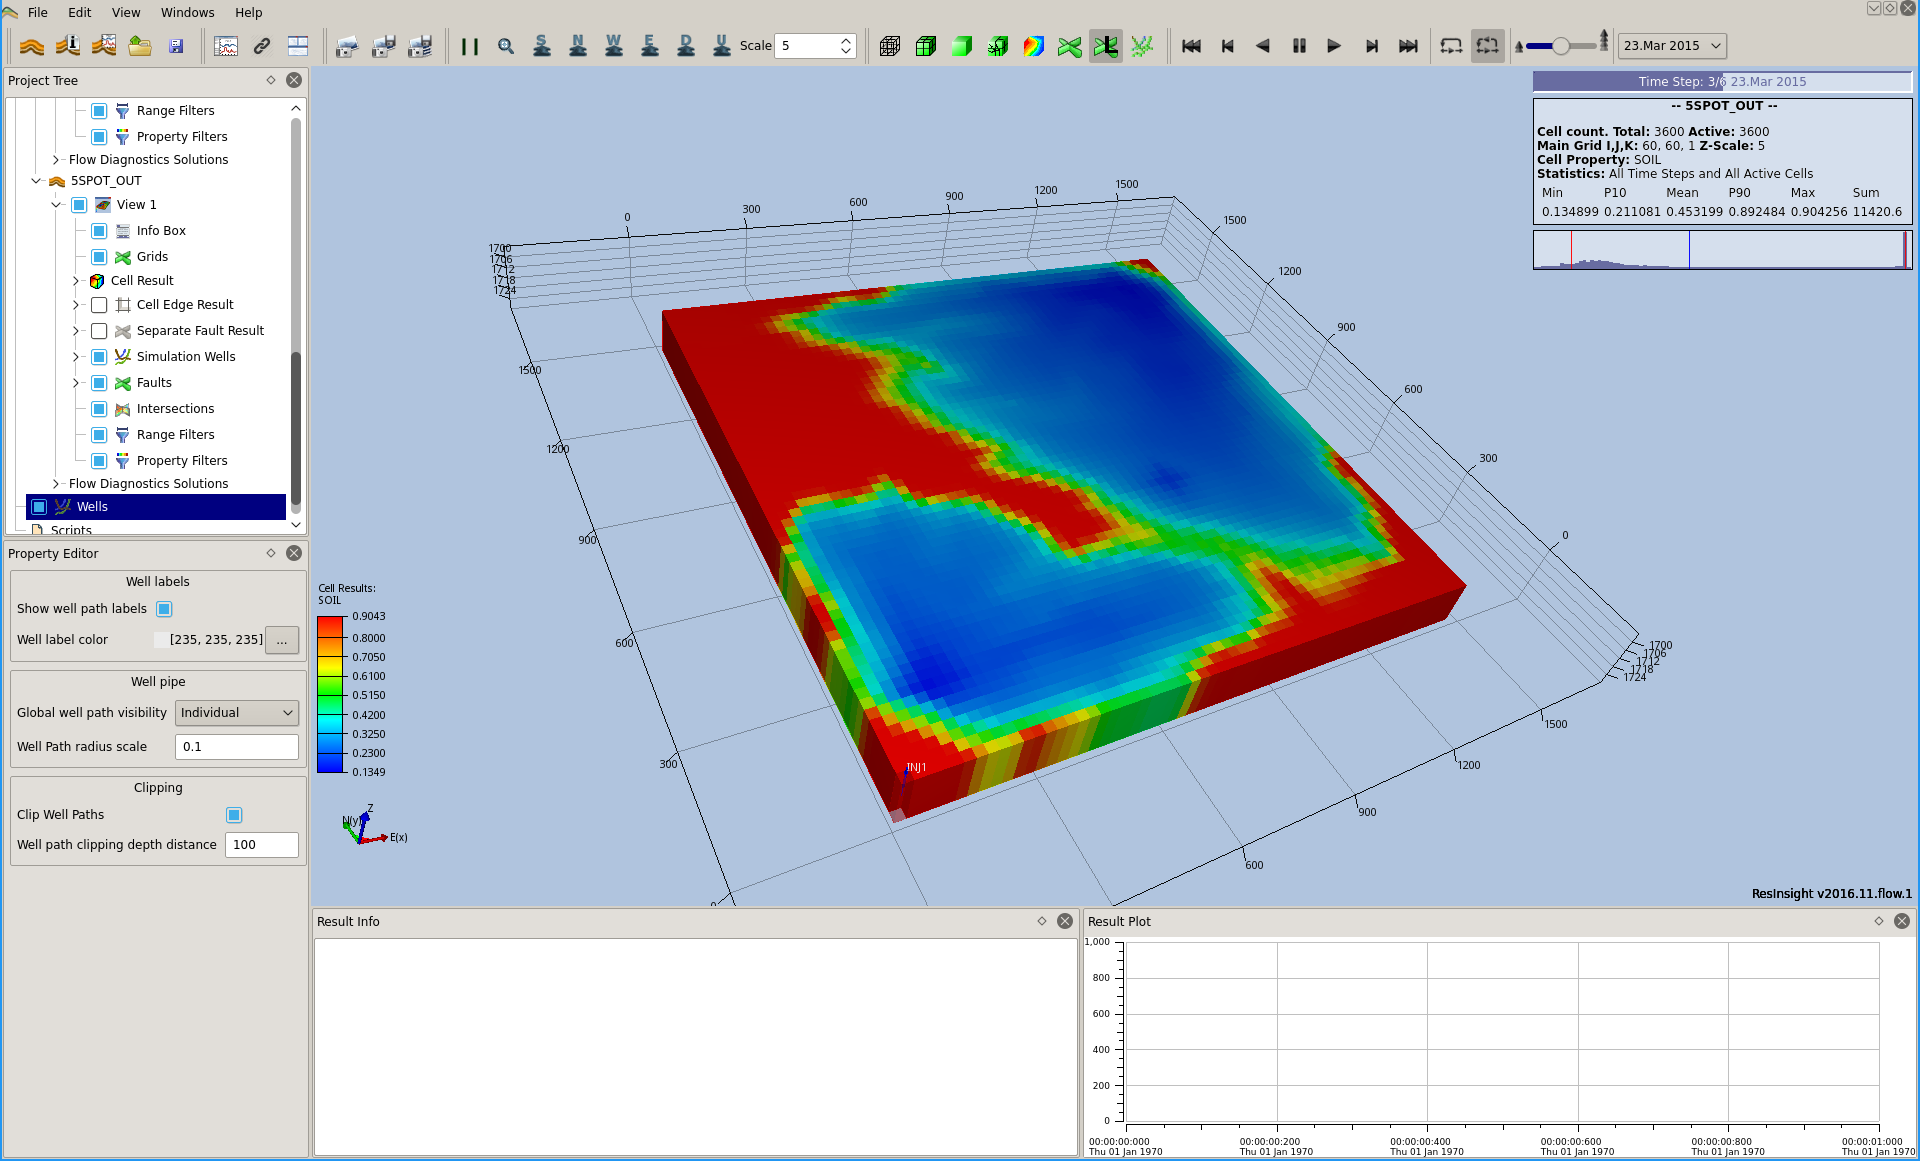
\includegraphics[scale=.25]{images/Screenshot-resinsight-5spot-soil.png}
\end{figure}

\begin{figure}[h!]
\centering
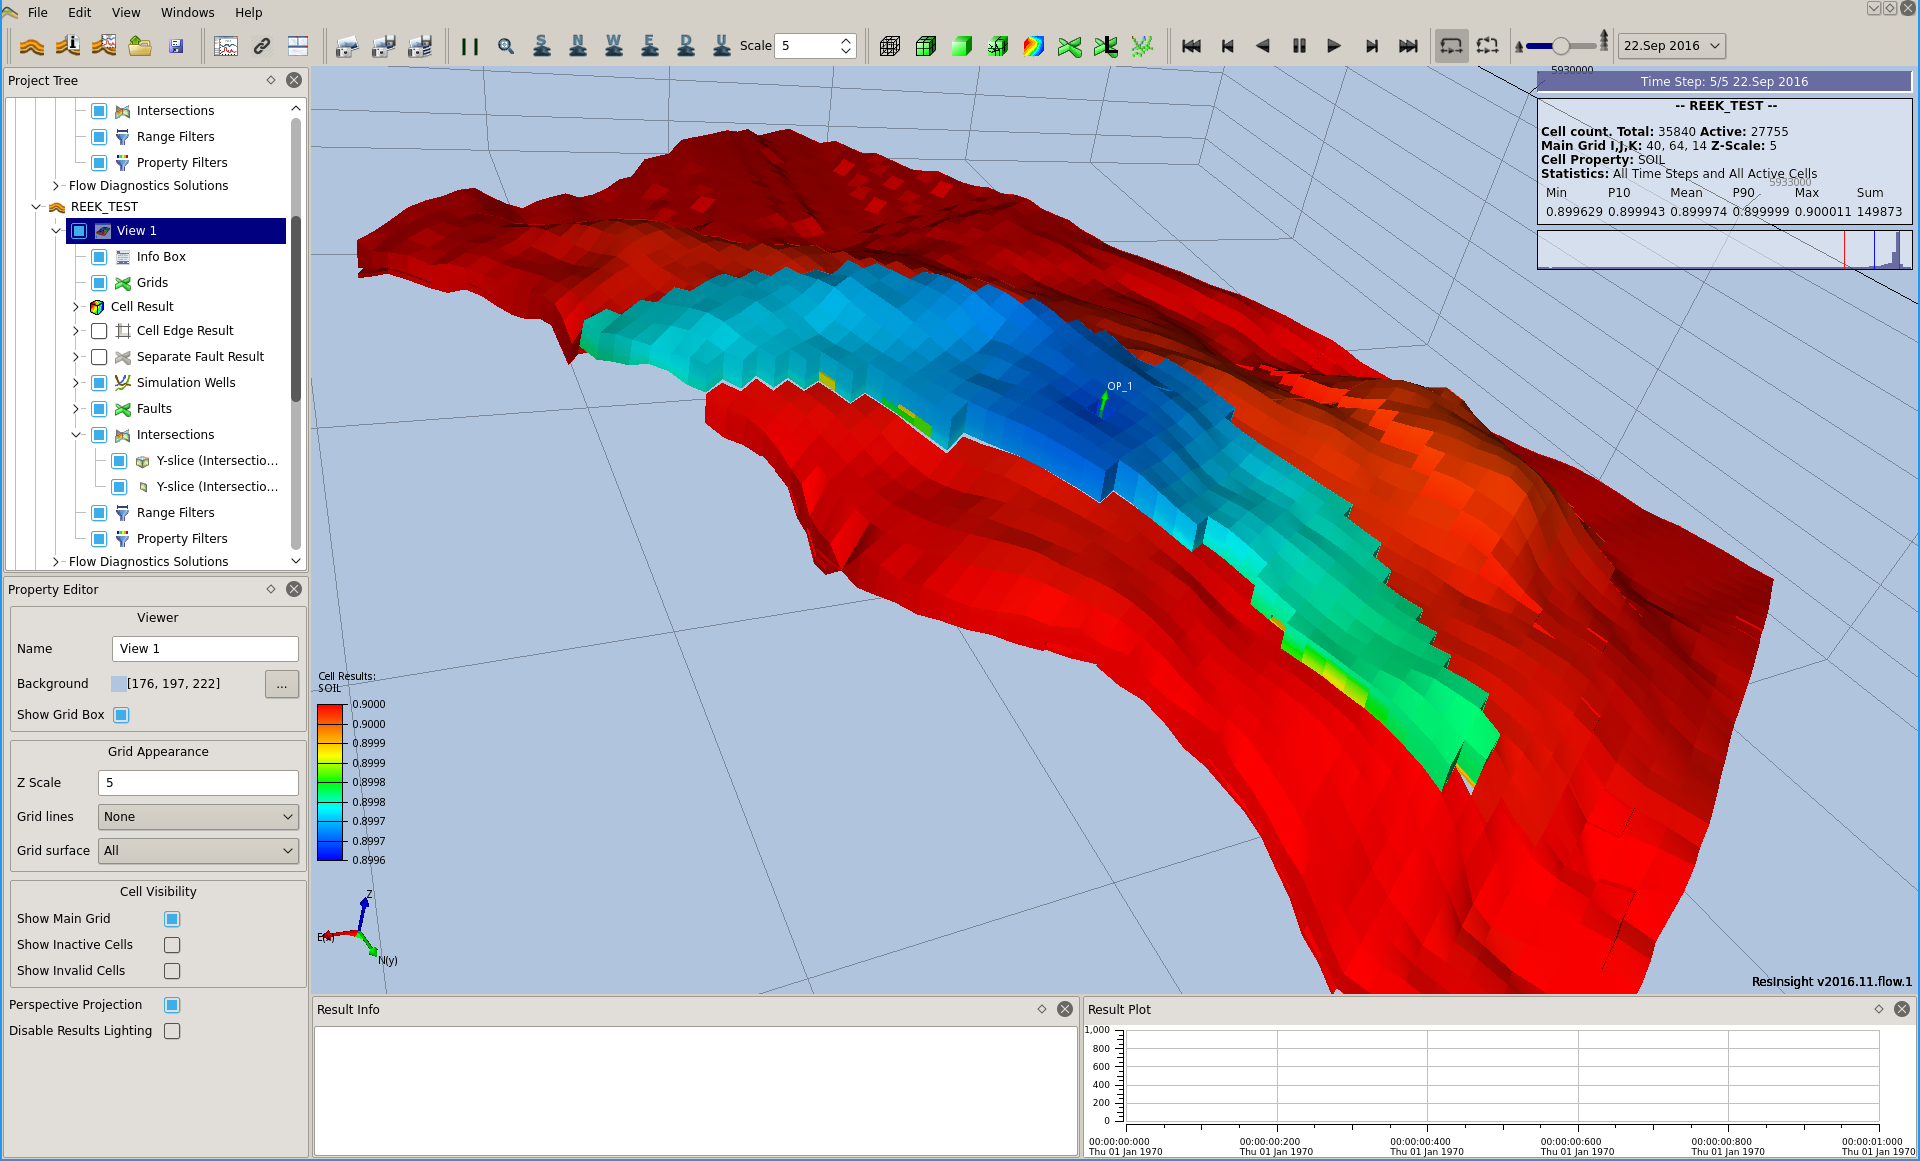
\includegraphics[scale=.25]{images/Screenshot-resinsight-reek-soil.png}
\end{figure}
\vspace{30mm}

\begin{figure}[h!]
\centering
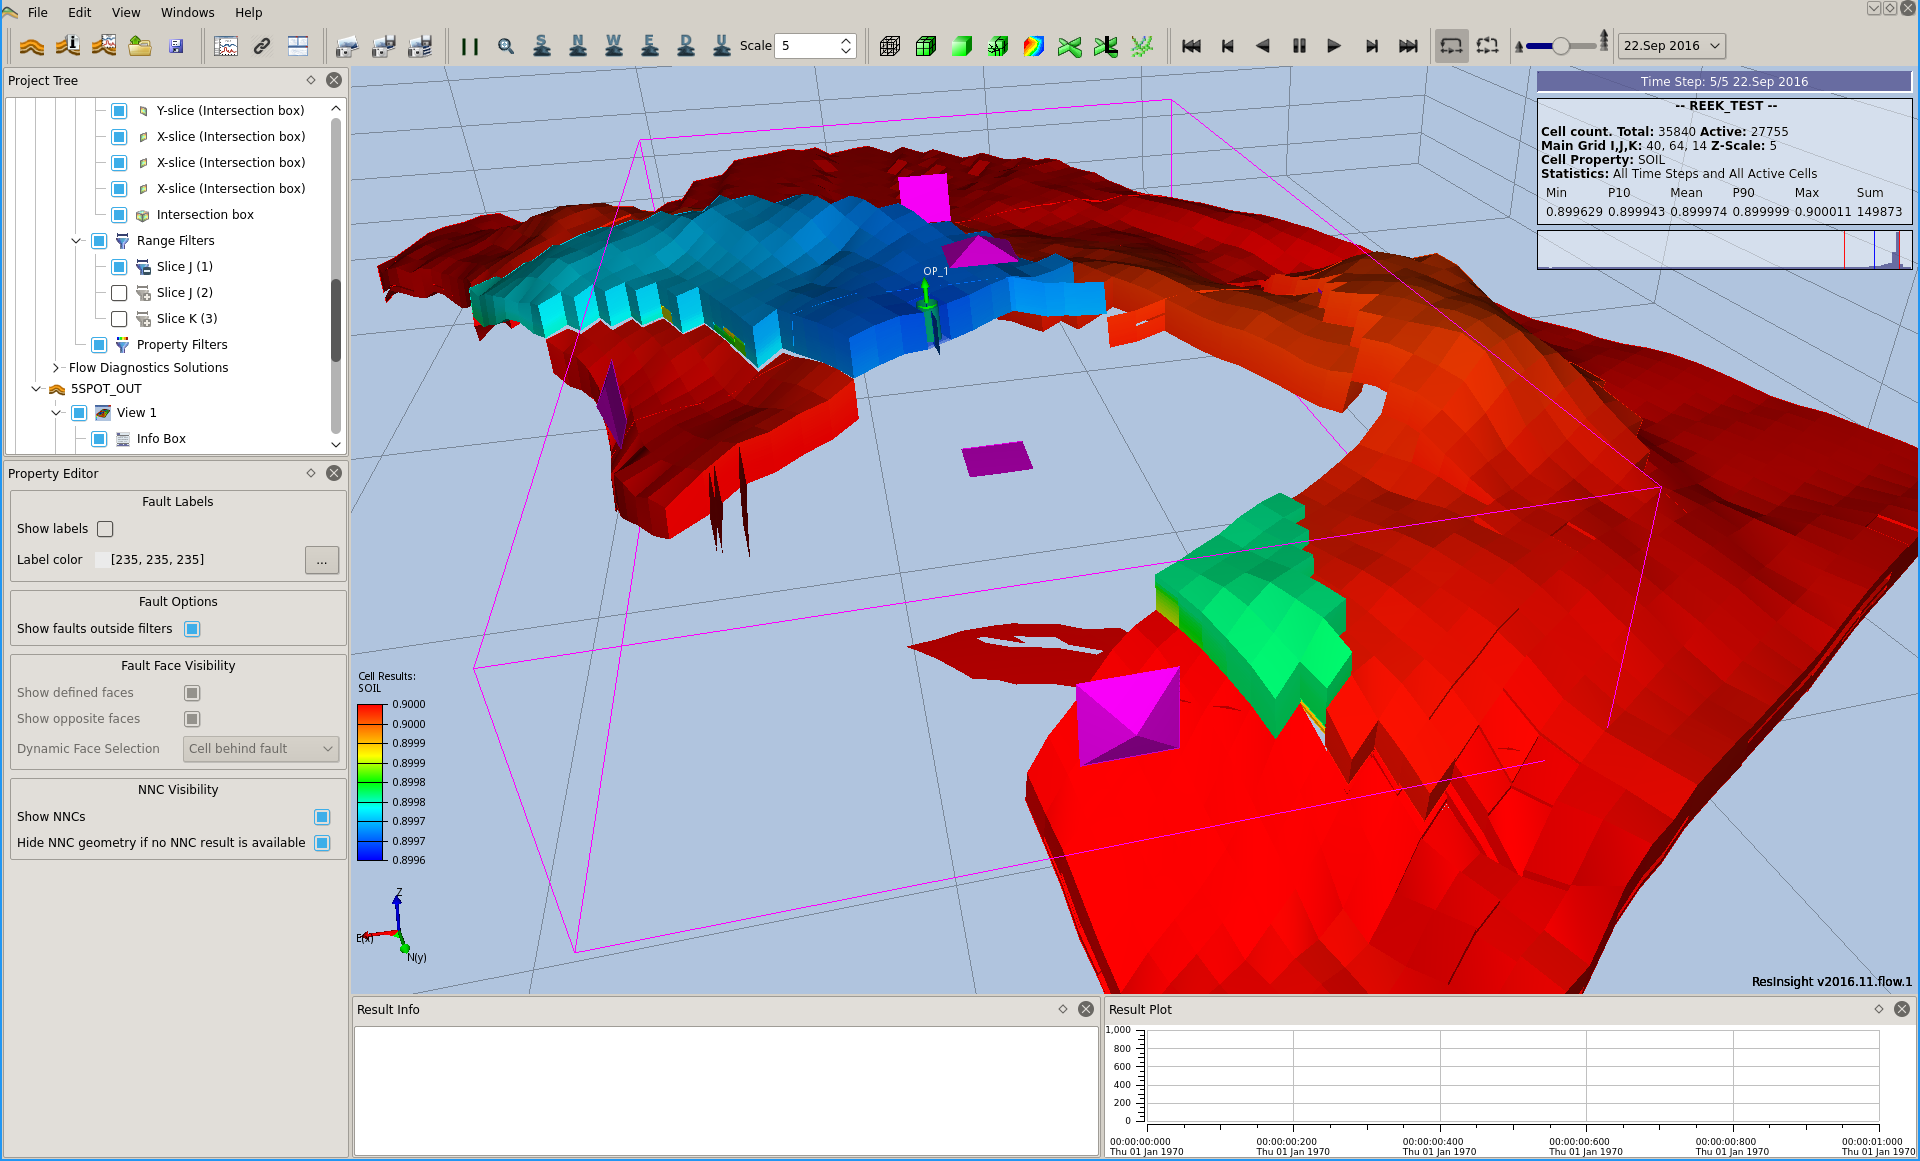
\includegraphics[scale=.25]{images/Screenshot-resinsight-reek-soil-range-filters.png}
\end{figure}


% % =============================================
% \subsection{...}



% ---------------------------------------------
% \subsubsection{}


 %\clearpage



% **********************************************************

% ----------------------------------------------------------


% ==========================================================
% REFERENCES
% \bibliographystyle{plainnatnourl}
% 
% LOCAL FROM REMOTE:
% \bibliography{bibsonomy_remote.bib}
% 
% GLOBAL FROM REMOTE:
% \bibliography{/home/bellout/Dropbox/WORK/H-WORKSPACE-A/%
% REORG_Literature/bib_files/bibsonomy_global_20160217.bib}

\end{document}